
W tej sekcji ukazujemy fragmenty kodu aplikacji klienta napisanych w języku Java.

\subsection{AudioConstants}
Klasa przechowująca stałe wykorzystywane do odbioru jak i przesyłania dzwięku w postaci bajtów.

\begin{figure}[H]
	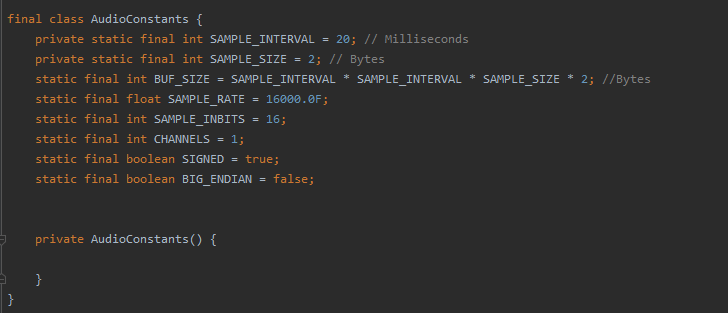
\includegraphics[width=\textwidth]{images/code3_1.png}
	\centering	
	\caption{\centering Stałe wykorzystywane przy cyfrowej obróbce dzwięku.}
\end{figure}


\subsection{BasicMicRegister}
Konstruktor tworzący obiekty potrzebne do otrzymywania jak i wysyłania dzwięku z mikrofonu jak i do szyfrowania i deszyfrowania ciągu bitów.

\begin{figure}[H]
	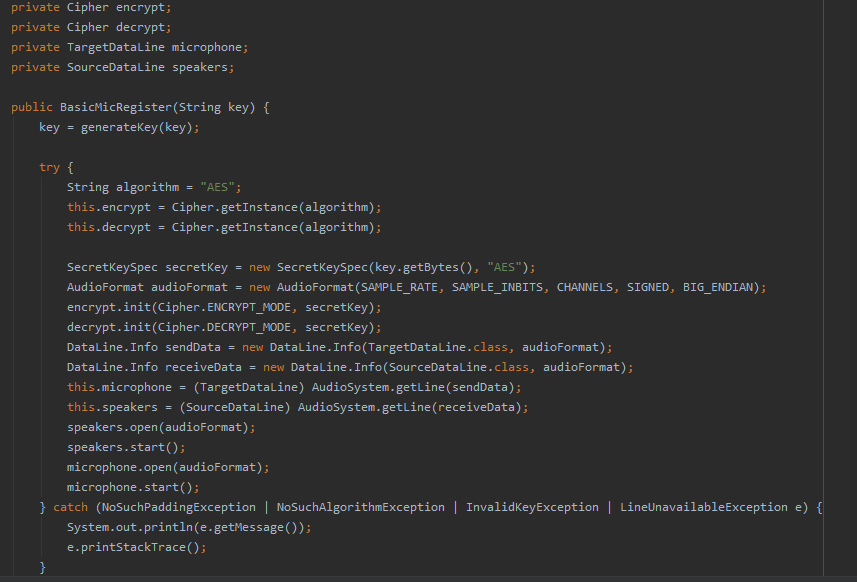
\includegraphics[width=\textwidth]{images/code4.png}
	\centering	
	\caption{\centering Konstruktor BasicMicRegister.}
\end{figure}


\subsection{sendVoiceMessage}
Metoda odpowiedzialna za przesyłanie zaszyfrowanej wiadomości głosowej uprzednio ustalonym kluczem szyfru blokowego AES 256.

\begin{figure}[H]
	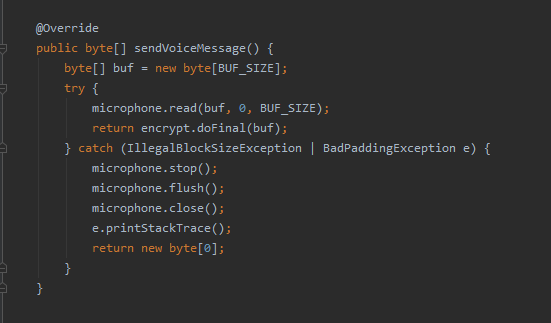
\includegraphics[width=\textwidth]{images/code5.png}
	\centering	
	\caption{\centering Metoda odpowiedzialna za przesyłanie zaszyfrowanej wiadomości.}
\end{figure}

\subsection{receiveMessage}
Metoda odpowiedzialna za odbieranie zaszyfrowanej wiadomości głosowej oraz odszyfrowanie jej i przekazaniu jej głośnikowi w celu odtworzenia dzwięku.
\begin{figure}[H]
	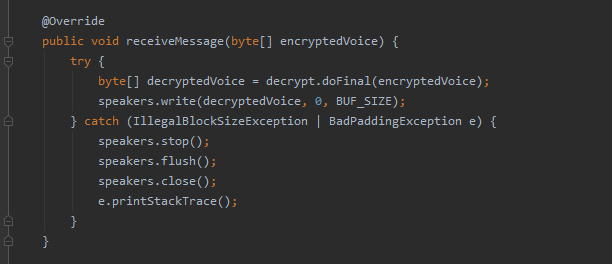
\includegraphics[width=\textwidth]{images/code6.png}
	\centering	
	\caption{\centering Metoda receiveMessage.}
\end{figure}